\documentclass[11pt]{extarticle}
\usepackage{manualdoprofessor}
\usepackage{fichatecnica}
\usepackage{lipsum,media9}
\usepackage[justification=raggedright]{caption}
\usepackage[one]{bncc}
\usepackage[acorde]{../edlab}
\usepackage{marginnote}
\usepackage{pdfpages}
\usepackage[printwatermark]{xwatermark}
%\newwatermark[pagex=2]{
\includegraphics[scale=3.3]{watermarks/test-a.png}}	% página específica
%\newwatermark[oddpages]{
\includegraphics{watermarks/test-a.png}}			% páginas ímpars
%\newwatermark[evenpages]{
\includegraphics{watermarks/test-a.png}}			% págimas pares
%\newwatermark[allpages]{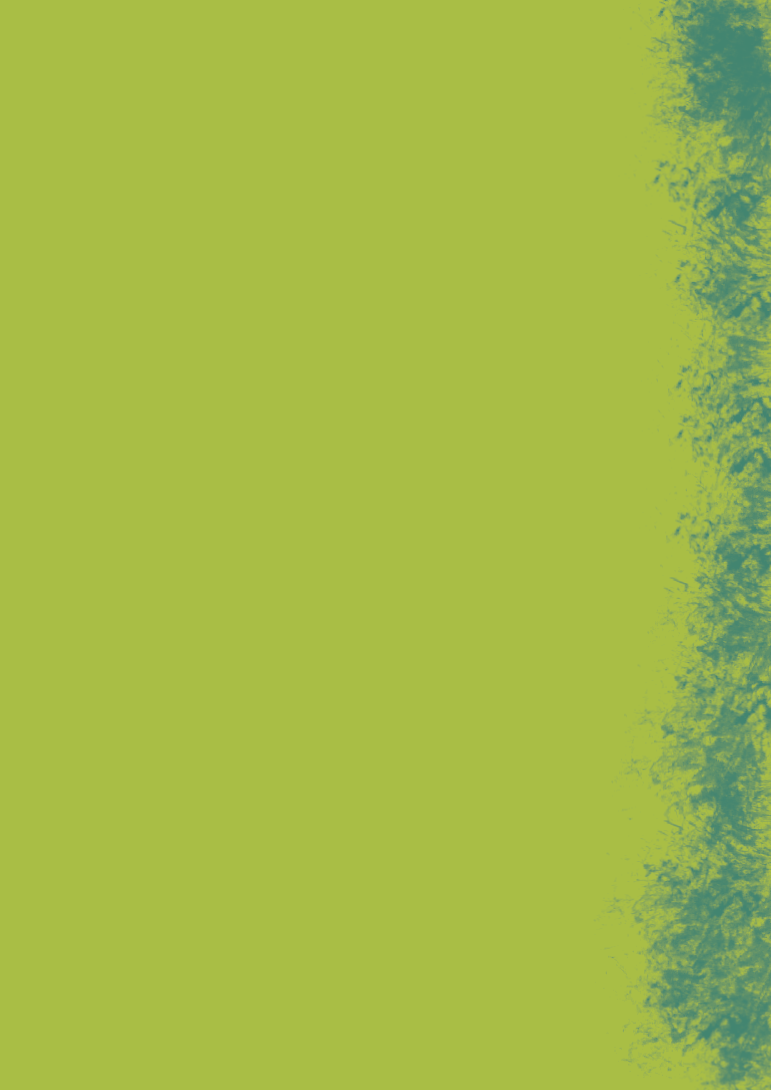
\includegraphics[scale=3.3]{watermarks/test-b.png}}
%\pagecolor{cyan!0!magenta!10!yellow!28!black!28!}

\newcommand{\AutorLivro}{Karel Capek}
\newcommand{\TituloLivro}{A fábrica de robôs}
\newcommand{\Genero}{Teatro}
%\newcommand{\imagemCapa}{./images/PNLD0001-01.png}
\newcommand{\issnppub}{978-65-99441-24-0}
\newcommand{\issnepub}{978-65-99441-27-1}
% \newcommand{\fichacatalografica}{PNLD0001-00.png}
\newcommand{\colaborador}{Gabriela Karam}

\begin{document}

\title{\TituloLivro}
\author{\AutorLivro}
\def\authornotes{\colaborador}

\date{}
\maketitle

%\begin{abstract}\addcontentsline{toc}{section}{Carta ao professor}
%\pagebreak

\tableofcontents

\section{Carta ao professor}

Caras e caros professores,

Este material tem a intenção de contribuir para que você consiga desenvolver um trabalho aprofundado com a obra \textit{A fábrica de robôs} em sala de aula. A obra traz diversos conceitos com base na discussão do progresso pela criação e evolução das máquinas através da tecnologia e ciência. Essa história é escrita na forma de texto teatral, que se apresenta com diálogos entre as personagens e algumas observações no corpo do texto, como o lugar onde as cenas acontecem, as rubricas de interpretação e de movimento, assim como os atos que dividem as cenas (uma espécie de capítulos). A leitura de uma peça teatral possibilita diversas atividades com os estudantes: desde a divisão em grupos que poderão ler o mesmo personagem em coro, até a montagem de cada ato com um grupo diferente de crianças, para que os alunos experimentem em seus corpos a vivência de diversos personagens. Além disso, o educador tem, com o texto teatral, a liberdade de mudar de tempos em tempos os alunos participantes da leitura dramatizada. O momento da leitura de peças teatrais costuma vir carregado de muita diversão para os alunos e provoca, como consequência do envolvimento com o texto, o entendimento da história e das questões levantadas por ela. Isso ocorre de forma natural e contínua ao longo da atividade. Além disso, brincar de ser uma personagem é algo que leva as pessoas para universos ainda não adentrados de sua vida, provocando soltura, trabalhando a timidez e gerando uma boa aceitação de si mesmo no mundo.

E para que todo esse trabalho artístico se torne possível com pensamento crítico, é interessante que falemos sobre o contexto do autor de \textit{A fábrica de Robôs}. Karel Capek (pronuncia-se Tchápek), nascido na então Austro-Hungria, hoje República Tcheca, foi um típico homem de seu tempo (1890-1938). Estava no meio da efervescência da Segunda Revolução Industrial, com a ascensão do pensamento liberal e por isso buscava ter o pensamento livre em suas obras, sempre com referência às questões de seu tempo e também se utilizando do pensamento distópico, ou seja, imaginava o que aconteceria em meio a tantas transformações econômicas e políticas, bem como os avanços tecnológicos que varriam os séculos XIX e XX. Capek tornou-se o máximo representante da cultura democrática de seu país, advertindo os compatriotas e o mundo a respeito do perigo dos fundamentalismos ideológicos, que varreriam a democracia e a cultura humanística tanto do velho continente quanto de qualquer outro ponto do mapa. Muito antes de a ficção científica ter sido reconhecida como gênero literário independente, Karel abordou questões seminais referentes à evolução do ser humano no planeta. Tinha inquietações acerca das consequências que tantos avanços poderiam provocar. Muitas de suas obras discutem os aspectos éticos e limitantes das invenções que marcaram o século passado e, além de colocar em relevo assuntos como a produção de armas nucleares ou modos de inteligência pós-humana, expressou considerável receio em relação a desastres futuros na Europa e no mundo, tais como violência e poderes ilimitados das grandes corporações e regimes tirânicos. Todas essas reflexões estavam alicerçadas na tentativa de vislumbrar meios para salvar a humanidade da autodestruição. 

\Image{Karel Capek (Portal da literatura; Domínio público)}{PNLD2023-021-02.png}

Uma vez que estamos trabalhando com estudantes de 4º e 5º ano, é interessante dizer que, por conta das densas informações presentes na peça, é sugerido ao educador que seja trabalhado na turma apenas o primeiro ato da peça, que carrega muito conteúdo em si e proporciona diversas possibilidades de jogos, reflexões e brincadeiras com a turma. No texto \textit{A fábrica de robôs}, que foi escrito em 1920 e logo acaba sendo traduzido para o inglês em 1923 - fato que impulsiona o rápido reconhecimento internacional  -, Karel discorre a respeito de seres artificiais, trabalhadores incansáveis e infalíveis, desprovidos de todas as “qualidades desnecessárias” que marcam os seres humanos, ou seja, não possuem criatividade alguma, não sentem dor nem possuem qualquer espécie de sentimento. Nessa sociedade, os robôs acabam assumindo todos e quaisquer encargos humanos, enquanto a vida humana torna-se banal, monótona, quase sem horizontes.

Há uma série de questões importantes a analisar, como o bônus e o ônus que a humanidade enfrentaria como resultado de um invento revolucionário como os robôs - situação que já está acontecendo sem ser levada ao limite como na obra -, bem como a problematização das redes sociais e os computadores, questionando se utilizamos de maneira adequada e como poderíamos repensar determinadas maneiras de uso da tecnologia. Uma das questões centrais que podem ser trabalhadas com a turma é o debate sobre o prejuízo que as tecnologias provocam na nossa atenção, que nos proporcionaria contemplar e até apreciar a arte e a leitura, mas está sendo prejudicada pela relação humana com os inventos tecnológicos contemporâneos. Cabe a pergunta: o que mudou com a presença do eletrônico que mais está presente no dia a dia, o celular, um aparelho que cumpre o papel de ser uma extensão do nosso corpo (como um braço de um robô ou até mesmo um cérebro)? 

\Image{Promovendo uma série de questões importantes de serem trabalhadas, como o bônus e o ônus que a humanidade enfrentaria como resultado de um invento revolucionário como os robôs (Instituto Conectomus; Domínio público)}{PNLD2023-021-03.png}

\section{Sobre o livro}

\textit{A Fábrica de Robôs} causou alarde quando foi encenada pela primeira vez, em 1921. Divida em três atos, a peça traz à tona uma temática incomum à época: a profunda crise deflagrada pelo avanço científico-tecnológico, a qual põe em risco a espécie humana. Após ganharem vida, máquinas semelhantes a seres humanos passam a exercer todas as atividades braçais, o que levou o homem a cunhar o termo “robô” – palavra que em tcheco significa servidão e trabalho forçado. Embora mais eficientes dentro da lógica capitalista, as tais máquinas desconhecem a criatividade e os sentimentos, o que acarreta consequências nefastas à humanidade, que acaba se moldando à lógica da produtividade. A peça traz a história de um cientista que descobre uma fórmula capaz de dar vida a máquinas de aparência humana, gerando um desequilíbrio radical no modo de produção e tornando a mão de obra humana obsoleta. Essas criaturas artificiais, desprovidas de sentimentos e criatividade, passam a exercer todas as atividades braçais, com consequências negativas para os homens. A palavra \textit{robô}, cujo significado em tcheco é \textit{servidão, trabalho forçado}, e que seria incorporada em quase todas línguas, foi cunhada e usada pela primeira vez na peça de Tchápek.

\Image{A peça traz a história de um cientista que descobre uma fórmula capaz de dar vida a máquinas de aparência humana (Tiinside; Domínio público)}{PNLD2023-021-04.png}

\section{Sobre o autor}

Karel Capek (1890-1938) foi um escritor e filósofo tcheco, nascido em Malé Svatonovice, Boêmia, então parte do Império Austro-Húngaro. Suas obras de ficção denunciaram os perigos do confronto entre o homem e os avanços tecnológicos, os perigos que ameaçavam o mundo moderno se este se deixasse levar pelos excessos do materialismo e do mecanicismo. Estudou filosofia em diversas cidades européias até se estabelecer em Praga (1917), onde trabalhou como escritor e jornalista. Na literatura, embora tenha cultivado diversos gêneros, deve sua popularidade sobretudo a suas obras de ficção, suas utopias satíricas e filosóficas, traduzidas para muitos idiomas. Por alguns anos escreveu em parceria com o irmão Josef, como por exemplo em \textit{Krakonosova zahrada} (1918), coletânea de contos e narrativas de grande interesse humano. Nessa obra, numa estória em que humanidade se achava ameaçada por uma máquina de sua invenção, o \textit{robot}, cunhou a palavra que posteriormente popularizou-se pelo mundo inteiro como nome de uma unidade cibernética. Morreu em Praga e entre outras obras importantes ficaram a peça dramática \textit{R.U.R.} (1920), \textit{Hordubal} (1933), \textit{Povetron} (1934) e \textit{Obycejny zivot} (1934), as famosas sátiras \textit{Valka smloky} (1936) e a peça realista \textit{Bilá nemoc} (1937), em que conclamava o povo à solidariedade e à resistência contra o nazismo.

\section{Sobre o gênero}

O gênero \textbf{teatro} é uma forma literária normalmente constituída de diálogos entre personagens e destinada a ser encenada, não apenas lida. As peças teatrais, tais como as que conhecemos no mundo ocidental, surgiram na Grécia Antiga, através das mãos de grandes teatrólogos, como Ésquilo, Sófocles, Eurípedes e Aristófanes.

\section{Proposta de Atividades}
\subsection{Pré Leitura}

A seguir você encontrará a descrição de uma aula modelo como exemplo prático de exploração do livro com estudantes. Esta seção apresentará orientações sobre como organizar a sala de aula para receber os estudantes, exercitar a interação entre eles e prepará-los para que o momento da leitura tenha mais riqueza de conteúdo.

\paragraph{Tema} A tecnologia na vida humana

\paragraph{Conteúdo} Efeitos das tecnologias na vida humana, especialmente no trabalho 

\paragraph{Objetivo} Refletir e debater sobre efeitos positivos e negativos da crescente importância na vida humana 

\paragraph{Justificativa} Desde muito cedo, nossas crianças e jovens são incentivados a utilizar dispositivos tecnológicos, como computadores e telefones celulares. Esta atividade de pré-leitura promove a reflexão crítica a respeito dos benefícios desses aparelhos à vida humana, mas também enfatiza os danos que podem ser causados pelo uso excessivo e deletério desses aparelhos.  

\paragraph{Metodologia} Antes de mergulhar no texto teatral, o educador pode embarcar com os estudantes em uma pesquisa sobre as invenções das máquinas, que trouxeram benefícios para a humanidade, mas também uma série de dilemas. É interessante mostrar para os alunos como a precarização do trabalho no campo colaborou para um êxodo rural e uma povoação intensa do meio urbano - muitas vezes sem preparo para receber tantas pessoas sedentas por emprego. 

\BNCC{EF04HI05}%Relacionar os processos de ocupação do campo a intervenções na natureza, avaliando os resultados dessas intervenções.
\BNCC{EF04HI06} %Identificar as transformações ocorridas nos processos de deslocamento das pessoas e mercadorias, analisando as formas de adaptação ou marginalização.
\BNCC{EF05HI07} %Identificar os processos de produção, hierarquização e difusão dos marcos de memória e discutir a presença e/ou a ausência de diferentes grupos que compõem a sociedade na nomeação desses marcos de memória.
\BNCC{EF04LP15}%Distinguir fatos de opiniões/sugestões em textos (informativos, jornalísticos,publicitários etc.).

Para trazer tantos debates à tona, sugere-se que o professor divida a turma em dois grupos e entregue diferentes pesquisas para que façam a leitura em conjunto nos grupos, sentados no chão, em roda. Duas pesquisas são sugeridas: o artigo \textit{16 grandes descobertas tecnológicas que impactaram o rumo da humanidade: Parte II}, de Márcia Pimentel. Disponível em \url{http://multirio.rio.rj.gov.br/index.php/leia/reportagens-artigos/reportagens/16755-16-grandes-descobertas-tecnol\%C3\%B3gicas-que-impactaram-o-rumo-da-humanidade-parte-ii} Acesso em 10 dez. 2021; e a matéria \textit{10 inventores que se arrependeram de suas maiores criações}, de Vitor Paiva. Disponível em \url{https://www.hypeness.com.br/2017/03/selecao-hypeness-10-inventores-que-se-arrependeram-de-suas-maiores-criacoes/}, acesso em 10 dez. 2021. Acompanhe a leitura conjunta e tire possíveis dúvidas a respeito da linguagem  e do conteúdo dos textos. Incentive que os alunos utilizem seus celulares para pesquisarem assuntos relacionados também, como, por exemplo, a vida dos cientistas citados ou demais curiosidades que possam surgir. Aproveite o momento para falar sobre a importância de usarmos nossos aparelhos eletrônicos com a finalidade de pesquisar, e não apenas de se relacionar pelas redes sociais. Após a leitura e pesquisa sobre o tema, peça que cada grupo elabore três perguntas sobre o assunto, tomando como base o debate sobre tecnologia e suas possibilidades, lados bons, médios e ruins, desejos que eles tenham (como por exemplo, não se identificar tanto com o uso de algum invento, ou as questões ambientais implicadas nos usos). Depois que o momento de pesquisa se encerrar, incentive que os grupos apresentem um para a sala o que descobriram, bem como o processo de pesquisa e em que lugares o debate chegou, bem como as impressões sobre as descobertas. A ideia é que a atividade se paute em uma abertura do processo de cada grupo, buscando dar autonomia aos alunos quanto aos debates que os permearam ao longo da pesquisa. Além disso, é interessante que os alunos do grupo que não está apresentando também participem, como uma grande conversa aberta. Levante questões como as condições dos trabalhadores que antes estavam no campo e, com os novos inventos, precisaram migrar para o meio urbano. Como foi esse processo? Houve uma precarização na vida desses trabalhadores? A proposta, com a atividade, é levar a turma a pensar sobre os resultados dos inventos, bem como os processos que levaram a isso e a vida dos trabalhadores que participaram de tudo isso. 

Fique atento a todas as formas de expressão: os gestos, as falas, as 
expressões faciais, para onde olham\ldots{} tudo pode ser explorado durante a conversa. 
Demonstre curiosidade sobre eles, seja um ouvinte entusiasmado e incentive que eles 
conversem entre si. Faça perguntas e construa a resposta junto com as crianças. 

A seguir, algumas dicas que podem contribuir para que a interação verbal seja produtiva em sua sala de aula: 

\begin{enumerate}
\item Sente-se no chão e participe com eles, trazendo pontos de vista a partir do que for trazido.

\item Não se esqueça que a conversa é uma troca e, portanto, evite ficar falando sozinho ou desvalorizar as respostas das 
crianças quando não conseguem formular frases completamente articuladas. Nunca descarte uma tentativa de comunicação. 

\item Evite utilizar falas negativas que desencorajam o diálogo. Se precisar que a turma corrija algum comportamento, explique claramente a razão e oriente com calma. Incentive positivamente as crianças e destaque o motivo de seus elogios sobre a forma de debate deles. 

\end{enumerate}

Depois que todos estiverem aquecidos com a discussão, sugere-se a promoção de um debate: o que poderia ser feito para que o trabalho do homem fosse aliviado e para que ele tivesse mais tempo para contemplação da vida? Que máquina poderia ser inventada para esse intento? Dividir a turma em grupos de cinco e cada um criar a sua própria invenção e fazer a exposição desse invento como se estivesse numa grande feira de tecnologia. No final, escolher qual invenção seria construída por uma fábrica mundial e todo mundo junto iria analisar os pontos positivos e negativos dessa invenção para os seres humanos.

\Image{Crianças prontas para a atividade (Tiinside; Domínio público)}{PNLD2023-021-05.png}


Outra consideração que pode ser feita sobre este tema é uma pesquisa sobre a época da industrialização desenfreada que ocorreu no mundo, levando milhares de pessoas a trabalharem em condições desumanas com a utilização de máquinas, que em princípio facilitaria as suas vidas nas fábricas, mas que, ao contrário, colocaram o ser humano ainda mais prejudicado e explorado a ponto de em 1811, na Inglaterra, uma manifestação de tecelões e artesãos ter sido severamente reprimida pelos policiais. Naquela noite, 60 teares foram destruídos por um grupo de manifestantes revoltados pelas más condições a que eram submetidos e as 17 horas de trabalho executadas pelos trabalhadores. Depois dessa pesquisa, o educador poderá mostrar trechos do filme \textit{Tempos modernos}, de Charles Chaplin, no qual o diretor utiliza a comédia para criticar esse sistema explorador, como faz nosso autor Karel Capek em seu texto teatral \textit{A fábrica de robôs}. Os trechos estão disponíveis no Youtube em \url{https://youtu.be/HglVC5bFqZ4}, \url{https://youtu.be/XLF1JZCxpxw} e \url{https://youtu.be/CjJplSmHfN8}. 

\Image{A industrialização e suas consequências (Cineset; Domínio público)}{PNLD2023-021-06.png}

Além disso, sugere-se a exibição do documentário \textit{2111: Robôs do futuro}, de Pablo Faivre (disponível no Youtube em \url{https://www.youtube.com/watch?v=gtUtczmJmO4}). O documentário fala a respeito das possibilidades de uma vida em que os robôs tenham inteligência artificial e as possíveis consequências disso. A partir daí, organize um debate sobre a opinião dos alunos acerca do assunto, provocando-os a abrirem suas opiniões e refletirem em conjunto sobre isso, aquecendo-os para a leitura da peça.

\paragraph{Tempo estimado} Quatro aulas de 50 minutos. 

\subsection{Leitura}

\paragraph{Tema} Leitura, compreensão e análise das personagens de \textit{A fábrica de robôs}

\paragraph{Conteúdo} Compreensão do texto e dos recursos teatrais.

\paragraph{Objetivo} Promover a leitura de \textit{A fábrica de robôs} e estimulá-la por meio de encenações. 

\paragraph{Justificativa} Além de colocar os estudantes em contato com o texto teatral, esta atividade lhes estimula a criatividade de maneira divertida, porque, depois de lerem o texto, eles devem \textit{criar}, ativamente, um diálogo improvisado entre uma personagem e um entrevistador, além de fazerem leituras dramáticas. Trata-se de uma atividade de leitura que escapa do formato tradicional e que pode ser muito estimulante, aproximando os estudantes do ambiente do teatro.         

Antes de partirmos para a leitura, é interessante ressaltar que a narrativa da ficção científica lida com conceitos ficcionais e imaginativos, relacionados ao futuro, ciência e tecnologia, e seus impactos e/ou consequências em uma determinada sociedade ou em seus indivíduos, desenvolvido no século XIX. Um dos marcos inicias da ficção científica é \textit{Frankenstein}, de Mary Shelley (1797-1851), publicado em 1818. Nessa obra, que se enquadra também no gênero terror, somos apresentados a um cientista que usa seus conhecimentos para criar um homem a partir de pedaços de pessoas mortas. É claro que o enredo vai além disso, mas é interessante ver o uso da ciência para promover coisas a princípio inimagináveis. Outra forma do uso da ficção científica, que teve grande repercussão nos anos 80, foi a viagem no tempo. Filmes como o \textit{Exterminador do futuro}, \textit{Em algum lugar do passado} e a trilogia \textit{De volta para o futuro}, mostravam esse desejo de exploração de teorias científicas reais. Esse tipo de filme nos obriga a refletir sobre a ciência e nos ajuda a desenvolver uma concepção menos cronológica do tempo (algo que a física já faz também). Outro filme de grande repercussão mundial é \textit{Star Wars}, que, em sua primeira versão, que estreou em 1977, teve a maior bilheteria de todos os tempos e concorreu ao Oscar daquele ano, mostrando que o nosso interesse pelos mistérios do futuro se intensifica conforme a passagem do tempo e os avanços tecnológicos que estamos presenciando. As perguntas acerca do futuro só aumentam. Por isso, ter conhecimento de \textit{A fábrica de robôs} é muito interessante para os alunos: para que seja externalizado o desejo de refletir sobre as possibilidades que o futuro pode reservar. Sendo assim, o educador pode se organizar para o momento da adentrar a obra em si.

\Image{Star Wars (Cineset; Domínio público)}{PNLD2023-021-07.png}

\paragraph{Metodologia} Antes da leitura propriamente dita, o educador pode ler o nome das personagens da peça e citar algumas características de cada uma delas.

PERSONAGENS 
HARRY DOMIN -  Diretor da fábrica Robôs Universais Rossum, na introdução com cerca de 38 anos, alto, sem barba.
 ENGENHEIRO FABRY -  Diretor técnico da R.U.R., também sem barba, loiro, sério e refinado. 
DR. GALL -  Supervisor do Departamento Fisiológico e de Pesquisas da R.U.R., miúdo, vivo, moreno, com bigode preto.
 DR. HALLEMEIER - Gerente do Instituto de Psicologia e Educação dos robôs, robusto, barulhento, com bigode ruivo inglês e cabelo ruivo cortado rente. 
CÔNSUL BUSMAN -  Diretor comercial da R.U.R., judeu gordo, calvo e míope. 
ENGENHEIRO CIVIL ALQUIST -  Supervisor de obras da R.U.R., mais velho do que os outros, desleixado no vestir, de cabelos e barba grisalhos e compridos. 
HELENA GLORY 
NANA - Sua governanta. 
MARIUS - Robô.
SULLA -  Robô
RADIUS – Robô
DAMON - Robô
PRIMUS - Robô
HELENA - Robô muito elegante

Veja as \textsc{bnccs} que estão relacionadas à atividade:

\BNCC{EF15AR18}%Reconhecer e apreciar formas distintas de manifestações do teatro presentes em diferentes contextos, aprendendo a ver e a ouvir histórias dramatizadas e cultivando a percepção, o imaginário, a capacidade de simbolizar e o repertório ficcional.
\BNCC{EF15AR20}%Experimentar o trabalho colaborativo, coletivo e autoral em improvisações teatrais e processos narrativos criativos em teatro, explorando desde a teatralidade dos gestos e das ações do cotidiano até elementos de diferentes matrizes estéticas e culturais.
\BNCC{EF15AR22}%Experimentar possibilidades criativas de movimento e de voz na criação de um personagem teatral, discutindo estereótipos.

A partir de então, sugerir uma atividade de entrevista com os estudantes. Coloca–se uma cadeira na frente da sala de aula e cada aluno, que já deve ter escolhido uma personagem para representar, se senta na cadeira e será entrevistado como se fosse a personagem. O educador irá conduzir a atividade fazendo perguntas sobre a personalidade e os desejos de cada uma e incentivando os alunos a responderem como se fossem cada uma dessas personagens.

\Image{sugerir uma atividade de entrevista com os estudantes (Nova escola; Domínio público)}{PNLD2023-021-08.png}

Depois desta atividade, os alunos já estarão mais inteirados com as personagens da peça e a leitura do texto poderá ser mais prazerosa e integrada. Peça que fiquem em roda e divida em grupos de personagens, assim poderão revezar para que todos os estudantes possam participar da leitura. Uma outra possibilidade de leitura também é criar coros que leiam ao mesmo tempo as personagens. Esta última possibilidade é interessante para que eles sintam a atmosfera de grupo que o teatro proporciona.

\paragraph{Tempo Estimado} Quatro aulas de 50 minutos. 

\subsection{Pós-leitura} 

\BNCC{EF15AR05}%Experimentar a criação em artes visuais de modo individual, coletivo e colaborativo, explorando diferentes espaços da escola e da comunidade.
\BNCC{EF35LP29}%Identificar, em narrativas, cenário, personagem central, conflito gerador, resolução e o ponto de vista com base no qual histórias são narradas, diferenciando narrativas em primeira e terceira pessoas.

\paragraph{Tema} Criação de narrativa. 

\paragraph{Conteúdo} Debate sobre dramatização, além de exercícios de encenação propriamente ditos. 

\paragraph{Objetivo} Estimular a capacidade criativa dos estudantes, além de promover esse trabalho em grupo, que exige cooperação e colaboração. 

\paragraph{Justificativa} Os exercícios teatrais propostos nesta atividade permitem aos estudantes a compreensão da importância do trabalho em grupo, além do aprofundamento nos conteúdos analisados nas atividades anteriores.   

Após a leitura, é interessante promover uma conversa sobre como os estudantes achavam que seria esse primeiro ato da peça, a partir da dramatização experimentada e também das entrevistas que foram feitas. Caso a peça tenha sido muito diferente do que eles achavam, pedir para que o novo enredo seja colocado para turma e os motivos pelos quais a nova narrativa foi proposta, para que todos entendam como uma história pode ser criada a partir de poucos elementos, como no caso desse primeiro ato da peça.

Depois deste momento, o professor poderá dividir a turma em grupos de cinco, dividir os momentos do ato lido e promover uma atividade em que cada grupo conte uma parte desse momento em forma de narrativa. Incentive-os a escolher nomes para o seu grupo que tenham a ver com a peça ou o tema da ficção científica. Dê um tempo para que eles dividam entre si as partes que irão contar, assim todos participarão da contação.

Posicione o grupo na frente da turma como se estivesse no teatro e apresente-os pelo nome, comunicando qual parte será feita, como se estivesse numa apresentação clássica de teatro, para dar início à narrativa de cada parte da história. No final das narrações, conduza-os para que cada grupo coloque no papel a sua parte. Estimule-os a usar desenhos e colagens para contar o seu trecho, mostre alguns livros que usam esses recursos para ajudar na melhor apreciação de uma história. Quando todos os grupos tiverem terminado, com a colaboração de todos, unam em conjunto as partes uma a uma, para que juntos formem um livro de história. Nesse momento ainda, pode se levantar a discussão sobre a diferença de uma peça teatral e uma história de um livro. Algo que pode ser pensado também é fazer o exercício inverso: trazer um livro de histórias e transformar numa peça teatral. 

\paragraph{Tempo Estimado} Quatro aulas de 50 minutos.   

\Image{Posicione o grupo na frente da turma como se estivesse no teatro (Crello; Domínio público)}{PNLD2023-021-09.png}

\section{Sugestões de referências complementares}

\subsection{Livros} 

\begin{itemize}
\item \textsc{huxley}, Aldous. \textit{Admirável mundo novo}. São Paulo: Boblioteca Azul, 2014.

Romance distópico que se utiliza da ficção científica para trazer um possível futuro em que a sociedade é completamente pautada em uma ciência que controla as atividades humanas e a natureza.  

\item \textsc{orwell}, George. \textit{1984}. São Paulo: Companhia das Letras, 2009.

Publicada originalmente em 1949, trata-se de uma distopia futurista, um dos romances mais influentes do século XX que provoca o leitor com a narrativa de uma sociedade a qual partidos políticos dominam a humanidade e controlam sua existência no mundo.

\item \textsc{bradbury}, Ray. \textit{Fahrenheit 451}. São Paulo: Boblioteca Azul, 2012.

Romance distópico sobre um bombeiro que tem como profissão atear fogo nos livros, em um mundo onde as pessoas vivem em função das telas a a literatura está ameaçada de extinção.

\end{itemize}

\subsection{Artigos}

\begin{itemize}
\item \textsc{pranke}, Marha Elfrida. Organização dos espaços da sala de aula na Educação Infantil. Disponível em: \url{http://centraldeinteligenciaacademica.blogspot.com/2016/04/organizacao-dos-espacos-da-sala-de-aula.html}. Acesso em 04 mai 2021. 

Artigo acadêmico que discorre sobre a importância da rotina e de criar ambientes dentro da sala de aula na Educação Infantil.

\item \textsc{morrell}, Andre Luiz Gioia, \textsc{morrell-junior}, Alexander Charles, \textsc{morrell}, Allan Gioia, \textsc{mendes}, Jose Mauricio Freitas, \textsc{tustumi}, Francisco e \textsc{silva}, Luiz Gustavo de Oliveira. Evolução e história da cirurgia robótica: da ilusão à realidade. Disponível em: \url{https://www.scielo.br/j/rcbc/a/4qVcw3NC75jwPNtkgkhwSWf/?lang=pt}. Acesso em 17 dez 2021. 

Artigo acadêmico que discorre sobre a ascensão da tecnologia robótica e a aplicação do uso de robôs na medicina. 
\end{itemize}

\subsection{\textit{Sites}}

\begin{itemize}
\item Vídeos “Conta pra mim” no site do PNA. Disponível em: \url{http://alfabetizacao.mec.gov.br/contapramim}. 
Acesso em 13 abr. de 2021.

Página do \textsc{mec} com vídeos sobre leitura dialogada que visam incentivar a Literacia Familiar. Muitas das técnicas, explicações e materiais disponíveis nessa página podem ser utilizados em aula, mas o site também pode ser uma ótima indicação para ajudar a direcionar os cuidadores dos estudantes a praticar a literacia familiar e leitura dialogada.

\item Artigo "Os robôs mais (e menos) inteligentes da ficção" da revista Super interessante. Disponível em: \url{https://super.abril.com.br/cultura/os-robos-mais-e-menos-inteligentes-da-ficcao/} Acesso em 17 dez. 2021. 

Neste artigo, a revista reuniu as máquinas mais célebres do cinema e da TV, provocando, de forma lúdica, o pensamento sobre os robôs das ficções.

\item Artigo "A ficção científica é a história do futuro. Mais respeito por ela", da revista Super interessante. Disponível em: \url{https://super.abril.com.br/ciencia/a-ficcao-cientifica-e-a-historia-do-futuro-mais-respeito-por-ela/}

O artigo da Super interessante provoca o debate de como a ficção científica por nos nortear e mesmo fazer com que problematizemos o resultado dos avanços científicos da contemporaneidade.

\end{itemize}

\section{Bibliografia comentada}

\subsection{Livros}

\begin{itemize}
\item \textsc{brasil}. Ministério da Educação. Base Nacional Comum Curricular. Brasília, 2018.

Consultar a \textsc{bncc} é essencial para criar atividades para a turma. Além de especificar quais habilidades precisam ser desenvolvidas em cada ano, é fonte de informações sobre o processo de aprendizagem infantil. 

\item \textsc{brasil}. Ministério da Educação. Secretaria de Alfabetização. Conta pra mim: Guia de Literacia Familiar. 
Brasília: \textsc{mec, sealf}, 2019. Disponível em: \url{http://alfabetizacao.mec.gov.br/images/conta-pra-mim/conta-pra-mim-literacia.pdf}.

Este guia é voltado aos pais e oferece explicações em uma linguagem bastante acessível e detalhada as práticas de Literacia Familiar, como praticar leitura dialogada, como narrar histórias, como exercitar interação oral, formas de proporcionar contatos com a escrita à criança etc. 
 
\item \textsc{wells}, Herbert George. Guerra dos mundos. São Paulo: Pé da Letra, 2016.

Uma história sobre a invasão da Terra por marcianos inteligentes, dotados de um poderoso raio carbonizador e máquinas assassinas, semelhantes a depósitos de água sobre tripés. Obra que dialoga com o universo da ficção científica.

\item \textsc{stanislavski}, Constantin. A preparação do ator. São Paulo: Civilização Brasileira, 1994.

Obra interessante para pesquisar a criação de personagens, bem como possibilidades de processos criativos no teatro. 

\item \textsc{cameron}, Julia. O caminho do artista. São Paulo: Sextante, 2017.

Livro que procura trazer ferramentas para despertar o potencial criativo e romper bloqueios.

\end{itemize}

\subsection{Filmes}

\begin{itemize}
\item \textit{Bacurau}. Dirigido por Kléber Mendonça Filho e Juliano Dornelles, 2019.

Num futuro próximo, Bacurau, uma pequena cidade brasileira no oeste de Pernambuco, lamenta a perda de sua matriarca, Carmelita (Lia de Itamaracá), que viveu até os 94 anos. Dias depois, seus habitantes aos poucos percebem algo estranho acontecer na região: enquanto drones passeiam pelos céus, estrangeiros chegam pela primeira vez na cidade com planos de exterminar toda a população ali residente, carros são atingidos por tiros e cadáveres começam a aparecer. Os habitantes chegam à conclusão de que estão sendo atacados. Resta identificar o inimigo e criar coletivamente um meio de defesa.

\item \textit{Matrix}. Dirigido por Lilly e Lana Wachowski, 1999. 

 filme descreve um futuro distópico no qual a realidade, como percebida pela maioria dos humanos, é, na verdade, uma realidade simulada chamada "Matrix", criada por máquinas sencientes para subjugar a população humana, enquanto o calor e a atividade elétrica de seus corpos são usados ​​como fonte de energia.

\item \textit{Elysium}. Dirigido por Neill Blomkamp, 2013.

Em 2154, uma pequena parte da população humana vive em Elysium, onde uma enorme estação espacial cria um habitat artificial disponível apenas para os mais ricos e onde qualquer doença ou ferimento são rapidamente curados em máquinas médicas. O resto da população mora na Terra, superpopulosa e pós-apocalíptica, decadente e patrulhada por robôs-policiais truculentos.

\end{itemize}

\end{document} 